\chapter{Modelling}
\label{ch:modelling}
After explaining thermal basics and the electrical analogy, the foundations are used in this chapter. The creation of the thermal model of the reference building and the resulting thermal model are presented. Later, the model is needed for the MPC to predict the thermal reactions of the building.

\section{The reference building}
\label{section:building}
    Since the thermal model and the MPC are based on a real building, details about the building are described below.
    \newline
    The building is located on the "Campus Nord" of the "Karlsruher Institut für Technologie (KIT)" and is part of the "Energy Lab 2.0", "a research infrastructure for renewable energy"\cite{KIT.2021}. It is equipped with a kitchen, a bathroom, five rooms and a technical room. For a better orientation, \autoref{fig:Bauplan} shows a part of the construction plan of the building. The building is designed as a single-family house, but for practical reasons, it is used as an office. The living area is around 100 $m^2$. The building offers two options to heat or cool with a ground-source heat pump or an air heat pump. The focus is on the air heat pump because the most commonly used heat pumps in Germany are air heat pumps \cite{bwp.2021}. In addition to the heat pump, there is a water reservoir for saving energy. The volume is 1000 litres \cite{Oskar}. However, the heating system is not completely installed yet. So heating or cooling is not possible actual.
    \newline
    One of the main features of the building is the number of sensors. The air temperature is measured in every room, as well as the temperature in the middle of the exterior wall, the screed temperature, the floor plate temperature, and the temperature of the inner wall between room three and room four (see \autoref{fig:Bauplan}). Furthermore, the consumption of the actual electrical power is also detected. Only the mentioned sensors are needed in this case, but there are many more sensors.
    %Himmelsrichtung noch beschreiben
    \begin{figure}
        \centering
        \def\svgwidth{320pt}
        \input{figure/Bauplan_WärmepumpenhausAuschnitt.pdf_tex}
        \caption{construction plan of the building \cite{Bauplan}}
        \label{fig:Bauplan}
    \end{figure}
    
\section{The thermal model}
\label{thermalmodel}
    %requirements
    The focus of this work is on the MPC part, so a simple thermal model is required. Nevertheless, no necessary information must be missing. Therefore, the thermal storage possibilities, the temperature inside of the building, and the heating system's influence have to be represented in the model. The storage allows to heat during the grid has too much power and to save the energy in the building during grid requires power. Hence, this enables the MPC's objective of grid services. The output of the model needs to be the temperature inside since the MPC aims to be in a pleasant temperature range to ensure customer comfort. Last, the influence of the heating system must be recognisable in the model, as it is the input of the plant.
    \newline
    The thermal model records the thermal conditions of the reference building. Therefore, the inner energy of the water reservoir and the air temperature inside the building are modelled. The water reservoir and the building behaviour are modelled according to different modelling strategies. The following chapters describe the partial models water reservoir and building model, the kind of modelling, and the conclusion of the partial models.
    
    
    \subsection{The modelling strategies}
    \label{ModellingStrategies}
    Creating a model can be made with three types of models, the so-called white-box models, grey-box models or black-box models. White-box models describe the real system only physically. Black-box models, on the other hand, have no physical description. They are created with data. And grey-box models are in between these two options \cite{Statusseminar.ForschungfurEnergieoptimiertesBauen.2009}. All possibilities are used in the thermal modelling of buildings \cite{Kramer.2012}.
    \newline
    The chosen approach for the MPC is the \textbf{grey-box model} for two reasons: First, this approach combines the advantages of white-box models and black-box models \cite{EstradaFlores.2006}. Second, there is the possibility to generate the required data from the reference building with the available measurement equipment at the KIT. According to Coakley et al., further advantages and disadvantages are among other things\cite{Coakley.2014}:
    \begin{table}[h!]
    \label{Advantages and disadvantages of grey-box modelling}
        \centering
        \begin{tabular}{p{7.3cm} | p{7.3cm}}
        \hline
          Advantages  &  Disadvantages\\
        \hline
        \begin{itemize}
            \item faster development by a combination of physical and statistical model
        \end{itemize}
      & \begin{itemize}
            \item requires knowledge in physical and statistical modelling 
        \end{itemize}\\
     \begin{itemize}
            \item accuracy of the results for the specific use case, provided by qualitative training data
        \end{itemize} & \begin{itemize}
            \item changes at the building lead to a re-training
        \end{itemize}\\
        \end{tabular}
        \caption {Advantages and disadvantages of grey-box modelling}
    \end{table}
    \newline
    However, the water reservoir and the heating system are not in use yet. So, no data are available for training a grey-box model. That's the reason why a part of the model needs to create as \textbf{white-box model}.
    \newline
    But also, white-box models have some pros and cons (see the following Table \cite{EstradaFlores.2006}).
    \begin{table}[]
    \label{tab:wihte-boxpro}
        \centering
        \begin{tabular}{p{7.3cm} | p{7.3cm}}
        \hline
          Advantages  &  Disadvantages\\
        \hline
        \begin{itemize}
            \item relies on physics
        \end{itemize}
      & \begin{itemize}
            \item needs assumptions to simplify 
        \end{itemize}\\
     \begin{itemize}
            \item applicable for every situation with the same assumptions and requirements 
        \end{itemize} & \begin{itemize}
            \item often complex mathematical problems
        \end{itemize}\\
        \end{tabular}
        \caption {Advantages and disadvantages of white-box modelling}
    \end{table}


    \subsection{The water reservoir model}
    \label{waterModel}
    First, all heat flows are regarded for modelling the water reservoir (WR), which influence the water reservoir (see \autoref{fig:Figure of the water reservoir with the heat flows}). The heat pump (HP) feeds the water reservoir with heat $\dot{Q}_\text{HP}$. The service water (SW) and the water for the heating circuit are taken from the storage. Since no service water is currently connected to the reference building, the heat flow $\dot{Q}_\text{SW}$ will be set to zero in the future. The heat losses $\dot{Q}_\text{loss}$ and the heating heat $\dot{Q}_\text{heating}$ are consequently the discharged heat. The resulting energy balance according to \autoref{eq:1HS} follows below.
    \begin{equation}
        \label{waterReservoir}
        \frac{d U_\text{WR}}{d t}= -\dot{Q}_\text{heating} + \dot{Q}_\text{HP} - \dot{Q}_\text{loss}
    \end{equation}
    
    \begin{figure}
        \centering
        \def\svgwidth{120pt}
        \input{figure/Wasserspeicher.pdf_tex}
        \caption{Figure of the water reservoir with the heat flows}
        \label{fig:Figure of the water reservoir with the heat flows}
    \end{figure}
    
    Since the model are referred to a real building, the size of the heat flows and the inner energy are limited according to the devices of the building. The heating heat moves in a range according to the calculations of the heating system \cite{Roth_Auslegung.2020} and can also have negative values when cooling is required (than according to the calculations of the cooling load \cite{SEFIngenieurgesellschaftMBH.2019}). The heat losses and the heat pump heat range are taken from the technical data \cite{Oskar}, \cite{TUM}.
    The maximal inner energy of the water reservoir is calculated according to \autoref{eq:innerEnergy} with the assumptions of a inlet temperature of 35°C and temperature spread of nine degree Celsius. The inlet temperature is chosen because the optimal inlet temperature for surface heating with heat pumps is around 35°C according to a heat pump manufacturer \cite{} and the temperature spread is taken from the calculations of the heating 

    \subsection{The building model}
    \label{building model}
    First, a physical description of the thermal dynamics of the building must be created. To obtain the condition of a simple model, we model the building as a single zone, as often practised in the literature \cite{Park.2011},\cite{Hazyuk.2012}. Single zone means that we sum all relevant values of the rooms, such as air temperature or wall temperature, by averaging to one value. 
    \newline
    We consider the air temperature, the temperature of the outer walls, the temperature of the inner walls and floors in the first floor, and the temperature of the floor in the model. In the following, these temperatures are called: inside temperature  $T_\text{inside}$, envelope temperature $T_\text{envelope}$, interior temperature $T_\text{interior}$, and floor temperature $T_\text{floor}$. 
    Using the state-space formulation (see \autoref{subsection:dynamics}), the temperatures are states in this model. According to the RC-analogy (see \autoref{electricalanalogy}), the model is built and nearly explained in the following for every state. \newline
    %\vspace{0.3cm}
    
    \textbf{Inside temperature:}\newline
    A focus lies on the accuracy of the inside temperature since this temperature will be controlled in the later prepared MPC. Therefore, a preciser description of the dynamics is required. We consider the influence of the sun $\dot{Q}_\text{sun,inside}$, the heating system $\dot{Q}_\text{heating}$ and the other states in the way shown in the following equation. $\dot{Q}_\text{heating}$  links the water reservoir model and the building model because the heat flow is the same but leaves the water reservoir model and enters the building model. 
    \begin{align}
        \label{eq:1.state}
        C_\text{inside}*\frac{d T_\text{inside}}{d t} &=& \dot{Q}_\text{heating} + \dot{Q}_\text{sun,inside} - \frac{T_\text{inside}-T_\text{envelope}}{R_\text{inside}} - \frac{T_\text{inside}-T_\text{outside}}{R_\text{window}} \\
       & &-\frac{T_\text{inside}-T_\text{interior}}{R_\text{interior}}-\frac{T_\text{inside}-T_\text{floor}}{R_\text{floor}}\nonumber
    \end{align}
    The detailed explanation for the composition of the thermal resistance and capacitance is in \autoref{electricalanalogy}. In the following, the special material and state dependant values are explained.
    The thermal capacitance $C_\text{inside}$ is calculated with the mass of the air from all rooms and the capacity of the air (1006 $J/(kg K)$ \cite{Weigand.2016}). The mass can be determined with the volume of the rooms according to the construction plan \cite{Bauplan} and the air density (1,28 $kg/m^3$ \cite{Weigand.2016}). 
    The thermal resistances $R_\text{inside}$ includes a convective part with the transfer coefficient $\alpha = 0,9 W/(m^2 K)$ special for air perpendicular to the wall in buildings with the assumption of a one Kelvin temperature difference between the wall and air \cite{Schweizer-fnalpha}.
    The window resistance $R_\text{window}$ is determined with the window area and the assumption of a heat transmission coefficient $u = 1 W/(m^2 K)$ \cite{ThorbenFrahm.2021}. 
    Heat conductivity and heat convection are the regarded mechanisms to determine the floor resistance $R_\text{floor}$. The floor material is reinforced concrete with the thermal conductivity of $2,3 W/(m K)$ \cite{AntonSchweizer.12.10.2021}. For the convection in the inner of the building, the same assumptions are made as for $R_\text{inside}$. 
    The interior resistance $R_\text{interior}$ is also calculated with the heat transfer coefficient inside.\newline 
    %\vspace{0.3cm}
    
    \textbf{Envelope Temperature:}\newline
    The sun, the contact of the walls with the inner air temperature and with the outside temperature influence the envelope temperature. The sun affects the air temperature in another area ratio than the outer walls. Therefore, we difference the influence of the sun on the inner air temperature and the envelope, and we consider here $\dot{Q}_\text{sun,envelope}$.  
    \begin{equation}
        C_\text{envelope}*\frac{d T_\text{envelope}}{d t} = \dot{Q}_\text{sun,envelope} - \frac{T_\text{envelope}-T_\text{outside}}{R_\text{envelope}} + \frac{T_\text{inside}-T_\text{envelope}}{R_\text{inside}}
    \end{equation}
    The outer wall resistance $R_\text{envelope}$ contains a heat conductivity of aerated concrete ($0,133 W/(m K)$ \cite{GhaziWakili.2015}) and the heat transfer coefficient for air perpendicular to the wall outside $\alpha_\text{envelope}$ according to the rules of thumb 
    \begin{equation}
        \alpha_\text{envelope} = 3,96 (v / L)^0,5 = 1,669 W/(m^2 K)
    \end{equation} from Schweizer-fn \cite{Schweizer-fnalpha}, with the average wind velocity of Karlsruhe $v$ \cite{AbteilungKlimaundUmweltberatung.2004} and the length of the building wall.
    To determine the capacitance $C_\text{envelope}$, we need the volume of the outer walls from the construction plan \cite{Bauplan}, the density of aerated concrete ($485 kg/m^3$) and the capacity (1000 $J/(kg K)$) \cite{GhaziWakili.2015}.\newline  
   % \vspace{0.3cm}
   
    \textbf{Interior and floor temperature:}\newline
    The differential equations for the interior and the floor temperature are so simple as possible. Both states have just an impact on the inside temperature. 
    Hazyuk et al. models for example also the ground floor as one state \cite{Hazyuk.2012}. The explanation is that the ground floor has no convective contact with the environment. Therefore, he is not modelled with the envelope for holding the physical structure, where the wind has an impact on the outer walls.
    The interior is extra modelled to improve the accuracy of the inside temperature equations because the capacitance of the inner walls is specially collected.
    \begin{align}
    C_\text{interior} \frac{d T_\text{interior}}{d t} &= \frac{T_\text{inside}-T_\text{interior}}{R_\text{interior}} \\
       C_\text{floor} \frac{d T_\text{floor}}{d t} &= \frac{T_\text{inside}-T_\text{floor}}{R_\text{floor}} \nonumber\\
    \end{align}
    As above, we need for the calculation of the capacitance $C_\text{floor}$ and $C_\text{interior}$ some material parameters. The material of the floor is reinforced concrete and the interior' material is aerated concrete. The previously unnamed material parameters are the density ($2500 kg/m^3$) \cite{AntonSchweizer.12.10.2021} and the capacity ($880 J/(kg K)$) \cite{AntonSchweizer.12.10.2021b} of reinforced concrete.\newline
     % \vspace{0.3cm}
     
    Summarising, \autoref{fig:structureThermalModel} illustrates the building model with its all connections according to the RC- analogy.
    \begin{figure}
            \centering
            \def\svgwidth{320pt}
            \input{figure/meinModel2.pdf_tex}
            \caption{structure of the thermal model in RC- analogy}
            \label{fig:structureThermalModel}
        \end{figure}
        
    \subsubsection{Parameter identification}
    \label{fig:WorkflowModel}
     \begin{figure}
            \centering
            \def\svgwidth{400pt}
            \input{figure/workflow greybox modelling.pdf_tex}
            \caption{Work flow of grey-box modelling with Matlab}
            \label{fig:structureThermalModel}
        \end{figure}
    \autoref{fig:workflow} explains the procedure, how to generate the grey-box model from the physical building model.\newline 
    The used toolbox from Matlab is the "System Identification Toolbox". For this application, the most important commands are "idgrey" and "greyest".
    With the idgrey-command, we can specify the building model as the initial model for the grey-box estimation in state-space formulation. That means the thermal resistances and capacitance, which we determined above, are the initial values for the estimation and they are the values, which the estimator from Matlab can vary. We add also the parameters $f_\text{sol,inside}$ and $f_\text{sol,envelope}$ for estimating because we model in the simplest way the heat flow of the sun isolation $\dot{Q}_\text{sun,envelope}$ and $\dot{Q}_\text{sun,inside}$ with the measured diffuse insolation $I_\text{sun}$. The initial values for $f_\text{sol,inside}$ and $f_\text{sol,envelope}$ are chosen as $0,25$ like Harb et al. \cite{Harb.2016}. 
    \begin{align}
       \label{eq:sun}
        \dot{Q}_\text{sun,inside} &= f_\text{sol,inside} I_\text{sun} \\
        \dot{Q}_\text{sun,envelope} &= f_\text{sol,envelope} I_\text{sun} \nonumber 
    \end{align}
    After that, we are looking for the data from the reference building. The data are generated in an experiment, but this is explained in a subsequent chapter. When we have the data, they are separated into training data and validation data. The training data are used for the estimation. From the reference building, we obtain the room temperatures, which we average with the capacitance of each room to one value, the inside temperature. The same procedure is adopted for the outer wall temperature, except that the outer wall temperatures are averaged with their own capacitance. The interior and the floor temperatures are determined in the same way. Also, we obtain data of the heating system for $\dot{Q}_\text{heating}$ and the weather specially the outside temperature $T_\text{outside}$ and the diffuse insolation $I_\text{sun}$ for determining $\dot{Q}_\text{sun,envelope}$ or $\dot{Q}_\text{sun,inside}$ \newline
    Now, the greyest- command executes the parameter identification with the training data (see in Appendix the initial values and the identified values) and we obtain the ready model.
    
    \subsubsection{Validation of the thermal model}
    \label{validationthermalmodel}

     \begin{figure}
            \centering
            \def\svgwidth{320pt}
            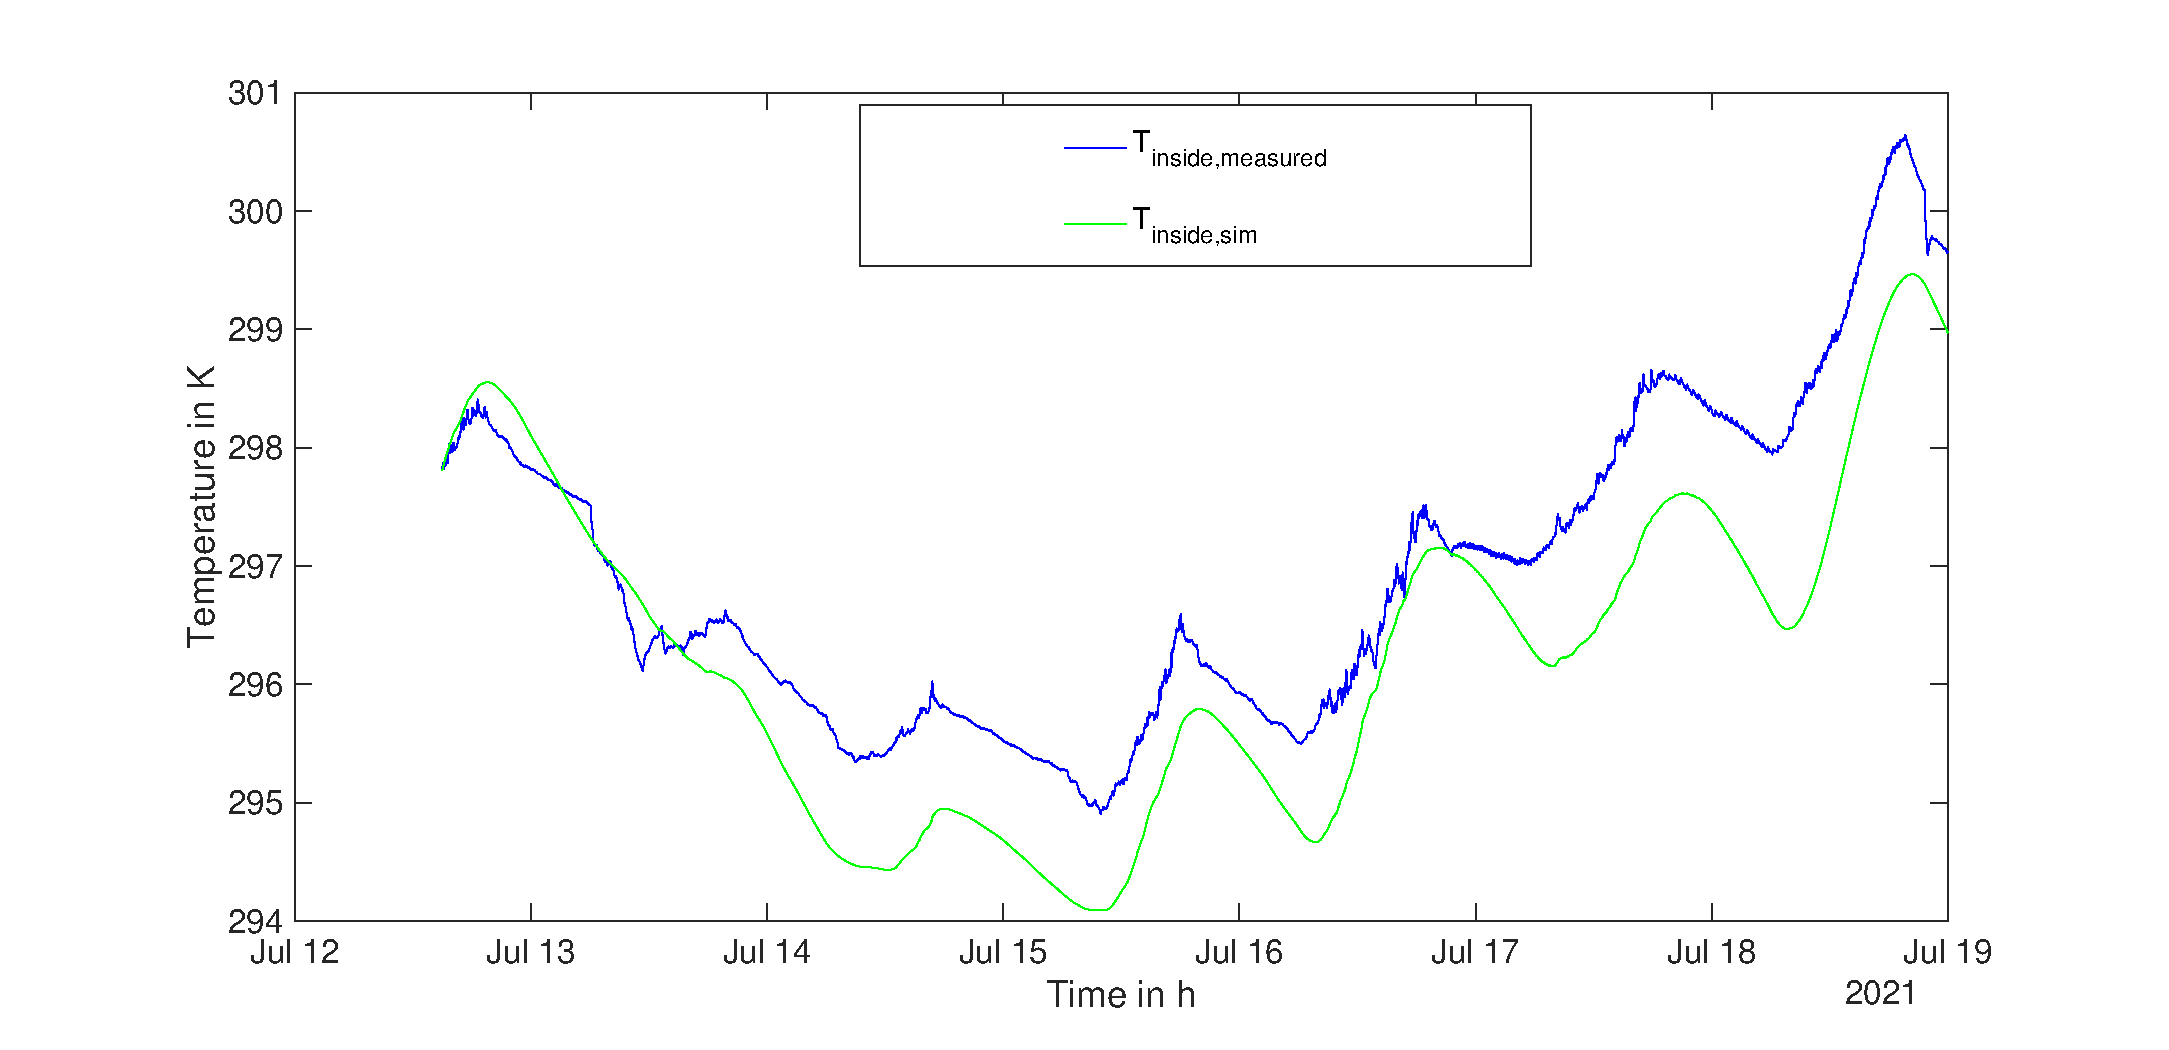
\includegraphics{figure/Verlauf_inside_ValidierungModell.eps}
           \caption{Validation of the building model}
           \label{fig:ValidationModel}
       \end{figure}
        
    \subsection{The hole model/Zustandsraumdarstellung}
    \label{holeModel}
    
\section{Experiment}
\label{thermalmodel}





%\begin{align}
  %% C_\text{inside}*\frac{d T_\text{inside}}{d t} &=& \dot{Q}_\text{heating} + \dot{Q}_\text{sun,inside} - \frac{T_\text{inside}-T_\text{envelope}}{R_\text{inside}} - \frac{T_\text{inside}-T_\text{outside}}{R_\text{window}} \\
       %& &-\frac{T_\text{inside}-T_\text{interior}}{R_\text{interior}}-\frac{T_\text{inside}-T_\text{floor}}{R_\text{floor}} \nonumber\\
      % C_\text{envelope}*\frac{d T_\text{envelope}}{d t} &=& \dot{Q}_\text{sun,envelope} - \frac{T_\text{envelope}-T_\text{outside}}{R_\text{envelope}} + \frac{T_\text{inside}-T_\text{envelope}}{R_\text{inside}} \nonumber \\
     %  C_\text{interior}*\frac{d T_\text{interior}}{d t} &=& \frac{T_\text{inside}-T_\text{interior}}{R_\text{interior}} \nonumber\\
    %   C_\text{floor}*\frac{d T_\text{floor}}{d t} &=& \frac{T_\text{inside}-T_\text{floor}}{R_\text{floor}} \nonumber\\
    %   \frac{d U_\text{WR}}{d t}&=& -\dot{Q}_\text{heating} + \dot{Q}_\text{HP} - \dot{Q}_\text{loss} - \dot{Q}_\text{SW} \nonumber
  %  \end{align}